% Fig. 1 (study sequence). Build: pdflatex fig1_workflow.tex
\documentclass[border=2pt]{standalone}
\usepackage[T1]{fontenc}
\usepackage{newtxtext}
\usepackage{tikz}
\usetikzlibrary{arrows.meta,calc}
\definecolor{cblue}{HTML}{2A78D6}
\definecolor{corange}{HTML}{EB6834}
\definecolor{caqua}{HTML}{1BAF7A}
\definecolor{cink}{HTML}{52514E}
\definecolor{cpurple}{HTML}{6A4C93}
\definecolor{fpurple}{HTML}{EFEAF5}
\begin{document}
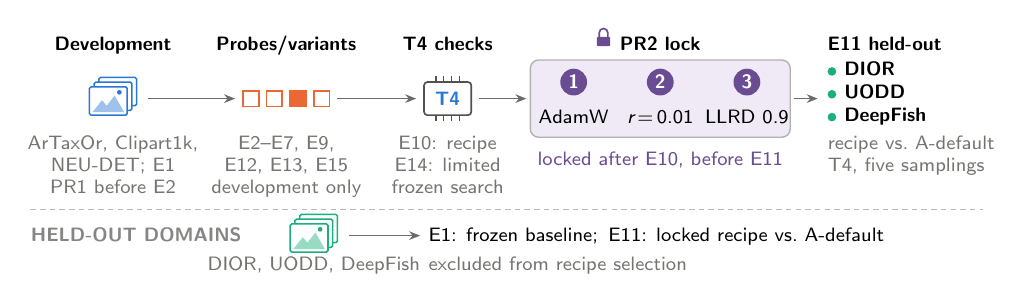
\begin{tikzpicture}[x=1cm,y=1cm,font=\sffamily\scriptsize,
  hdr/.style={font=\sffamily\scriptsize\bfseries,anchor=base,inner sep=0pt},
  sub/.style={text=cink!80,align=center,anchor=north,inner sep=0pt},
  arr/.style={-{Stealth[length=1.4mm,width=1.1mm]},draw=cink!85,line width=.5pt},
  num/.style={circle,fill=cpurple,text=white,font=\sffamily\scriptsize\bfseries,inner sep=0pt,minimum size=3.4mm},
  pics/tiles/.style={code={
    \foreach \d in {0.12,0.06,0}{\draw[#1,fill=white,line width=.55pt,rounded corners=.6pt] (-0.3+\d,-0.21+\d) rectangle (0.18+\d,0.15+\d);}
    \fill[#1!45] (-0.26,-0.17) -- (-0.14,-0.02) -- (-0.08,-0.09) -- (0.02,0.04) -- (0.14,-0.17) -- cycle;
    \fill[#1] (0.08,0.08) circle (0.03);}}]
\node[hdr] at (1.05,1.9) {Development};
\node[hdr] at (3.25,1.9) {Probes/variants};
\node[hdr] at (5.3,1.9) {T4 checks};
\node[hdr] (pr2h) at (8.0,1.9) {PR2 lock};
\node[hdr] at (10.85,1.9) {E11 held-out};
\begin{scope}[shift={($(pr2h.west)+(-0.2,0.06)$)}]
\draw[cpurple,line width=.6pt] (-0.055,0.02) -- (-0.055,0.08) arc (180:0:0.055) -- (0.055,0.02);
\fill[cpurple,rounded corners=.4pt] (-0.085,-0.09) rectangle (0.085,0.03);
\end{scope}
\pic at (1.05,1.29) {tiles=cblue};
\node[sub] at (1.05,0.82) {ArTaxOr, Clipart1k,\\NEU-DET; E1\\PR1 before E2};
\foreach \x in {2.8,3.1,3.7}{\draw[corange,line width=.6pt] (\x-0.1,1.19) rectangle (\x+0.1,1.39);}
\filldraw[corange,line width=.6pt] (3.3,1.19) rectangle (3.5,1.39);
\node[sub] at (3.25,0.82) {E2--E7, E9,\\E12, E13, E15\\development only};
\foreach \x in {5.15,5.25,5.35,5.45}{\draw[cink,line width=.5pt] (\x,1.5)--(\x,1.58) (\x,1.08)--(\x,1.0);}
\draw[cink,fill=white,line width=.6pt,rounded corners=1.2pt] (5.0,1.08) rectangle (5.6,1.5);
\node[font=\sffamily\scriptsize\bfseries,text=cblue] at (5.3,1.29) {T4};
\node[sub] at (5.3,0.82) {E10: recipe\\E14: limited\\frozen search};
\draw[cink!45,fill=fpurple,rounded corners=3pt,line width=.5pt] (6.35,0.8) rectangle (9.65,1.78);
\foreach \i/\x/\t in {1/6.9/AdamW,2/8.0/{{\itshape r}\,=\,0.01},3/9.1/LLRD 0.9}{
  \node[num] at (\x,1.5) {\i};
  \node[anchor=base,inner sep=0pt] at (\x,0.98) {\t};}
\node[text=cpurple,anchor=north,inner sep=0pt] at (8.0,0.62) {locked after E10, before E11};
\foreach \y/\t in {1.58/DIOR,1.29/UODD,1.0/DeepFish}{
  \fill[caqua] (10.18,\y+0.055) circle (0.055);
  \node[anchor=base west,inner sep=0pt,font=\sffamily\scriptsize\bfseries] at (10.33,\y) {\t};}
\node[sub,anchor=north west,align=left] at (10.12,0.82) {recipe vs.\ A-default\\T4, five samplings};
\draw[arr] (1.5,1.29)--(2.6,1.29);
\draw[arr] (3.9,1.29)--(4.9,1.29);
\draw[arr] (5.7,1.29)--(6.3,1.29);
\draw[arr] (9.7,1.29)--(10.0,1.29);
\draw[cink!40,line width=.5pt,dash pattern=on 2pt off 1.5pt] (0,-0.12)--(12.1,-0.12);
\node[anchor=base west,inner sep=0pt,font=\sffamily\scriptsize\bfseries,text=cink!70] at (0,-0.52) {HELD-OUT DOMAINS};
\pic at (3.6,-0.45) {tiles=caqua};
\draw[arr] (4.05,-0.45)--(4.95,-0.45);
\node[anchor=base west,inner sep=0pt] at (5.05,-0.52) {E1: frozen baseline;\enspace E11: locked recipe vs.\ A-default};
\node[sub,anchor=north west] at (5.05,-0.72) {excluded from recipe selection};
\node[sub] at (3.6,-0.72) {DIOR, UODD, DeepFish};
\end{tikzpicture}
\end{document}
